%% %%%%%%%%%%%%%%%%%%%%%%%%%%%%%%%%%%%%%%%%%%%%%%%%%
%% Template for a Chalmers KUL2023, version 1.0
%% by Samuel Bengmark
%% Developed from UF_FRED_paper by Ariel Soto-Caro
%% %%%%%%%%%%%%%%%%%%%%%%%%%%%%%%%%%%%%%%%%%%%%%%%%%

\documentclass[11pt]{article}
\usepackage{KUL_style}

\usepackage{lipsum}  %% Package to create dummy text (comment or erase before start)

%% ===============================================
%% Setting the line spacing (3 options: do not change)
% \doublespacing
 \singlespacing
% \onehalfspacing
%% ===============================================

\setlength{\droptitle}{-5em} %% Don't touch


% TITLE:
\title{Write your title here
\thanks{Presented at Chalmers Conference on Teaching and Learning 2023, KUL2023}
}

% AUTHORS:
\author{First Author\\% Name author
    \href{mailto:firstauthor@chalmers.se}{\texttt{firstauthor@chalmers.se}} %% Email author 1 
\and Second Author\\% Name author
    \href{mailto:secondauthor@chalmers.se}{\texttt{secondauthor@chalmers.se}} %% Email author 2
\and Third Author\\% Name author
    \href{mailto:thirdauthor@chalmers.se}{\texttt{thirdauthor@chalmers.se}}%% Email author 3
%\and Forth Author\\% Name author
%    \href{mailto:forthuthor@chalmers.se}{\texttt{forthuthor@chalmers.se}}%% Email author 4
    }
    
% DATE:
\date{\today}

% %%%%%%%%%%%%%%%%%%%%%%%%%%%%%%%%%%%%%%%%%%%%%%%%%%%%%%%%%%
% %%%%%%%%%%%%%%%%%%%%%%%%%%%%%%%%%%%%%%%%%%%%%%%%%%%%%%%%%%
\begin{document}

\maketitle
\pagenumbering{gobble}
% %%%%%%%%%%%%%%%%%%
\selectlanguage{american}
\begin{abstract}

Write your English abstract here. Max 150 words. The KUL proceedings will be bilingual. The main text can be written in either English or Swedish. Whatever language you choose you must include two abstracts, one in English and one in Swedish. %% Instructional text. Erase before use.

\lipsum[1] %% Dummy text for abstract. Erase before use.

\end{abstract}


\selectlanguage{swedish}
\begin{abstract}

Skriv ditt svenska abstrakt här. Max 150 ord. %% Instructional text. Erase before use.

\lipsum[1] %% Dummy text for abstract. Erase before use.


\end{abstract}
\selectlanguage{american} %% Choose the language you use for your main text. 
%\selectlanguage{swedish} 

%\noindent
\textit{\textbf{Keywords: }%
key1; key2; key3; key4.} \\ 


\section{Introduction}

The conference formats have different expectations and criteria, such as word limits, that must be followed. These can be found on \href{https://ui.ungpd.com/Issues/e0fb7d63-8d2c-4750-b0d7-eb92da240e1c?AccountId=8117a48b-bad0-418e-b612-2186302f6ab7&ContactId=21763c94-0f39-4710-b3df-4de5361ed673&IssueId=e0fb7d63-8d2c-4750-b0d7-eb92da240e1c&ir=e554dac0-c2a2-40f4-a314-28d3b3b50061}{\texttt{the website for KUL2023}}. The chapters in this template are suggestions, not mandatory.  %% Instructional text. Erase before use.

In this text follow the APA7 guidelines. For example, if the names of the authors are mentioned in the text the citation should look like \citet{Hardaker2004}. Otherwise it should look like \citep{Chavas2015}. %% Instructional text. Erase before use.

\lipsum[2-5] % Dummy text. Erase before writing.

\section{Methodology}

\lipsum[7-9] % Dummy text. Erase before writing.


\section{Results}

\lipsum[12-13] % Dummy text. Erase before writing.

\begin{table}[H] %% Instructional example of table. Erase before use.
  \centering
  \caption{Write a caption before the table, according to APA7.}
  \label{tab:1}
  \scalebox{.8}{
    \begin{tabular}{rlrrrrrr}
    \hline
    \multicolumn{1}{c}{\textbf{Variables}} & \multicolumn{1}{c}{\textbf{Categories}} & \multicolumn{1}{c}{\textbf{Unit}} & \multicolumn{1}{c}{\textbf{Rep}} & \multicolumn{1}{c}{\textbf{Mean}} & \multicolumn{1}{c}{\textbf{St. Dev.}} & \multicolumn{1}{c}{\textbf{Min}} & \multicolumn{1}{c}{\textbf{Max}} \\ \hline \hline

    \multicolumn{1}{l}{Variable 1} & Category A & \multicolumn{1}{c}{\$} & \multicolumn{1}{c}{8} & 0     & 0     & 0     & 0 \\
          & Category B & \multicolumn{1}{c}{lb} & \multicolumn{1}{c}{8} & 22,411.20 & 6,325.90 & 13,819 & 31,201 \\
          & Category C & \multicolumn{1}{c}{\$} & \multicolumn{1}{c}{8} & 5,869.60 & 4,609.90 & -464.1 & 12,744.10 \\
    \multicolumn{1}{l}{Variable 2} & Category A & \multicolumn{1}{c}{\$} & \multicolumn{1}{c}{8} & 1,777.40 & 144.5 & 1,642.30 & 1,912.60 \\
          & Category B & \multicolumn{1}{c}{lb} & \multicolumn{1}{c}{8} & 21,444.80 & 5,146.90 & 15,096 & 28,032 \\
          & Category C & \multicolumn{1}{c}{\$} & \multicolumn{1}{c}{8} & 4,138.50 & 2,644.10 & 22.2  & 7,932.70 \\
    \multicolumn{1}{l}{Variable 3} & Category A & \multicolumn{1}{c}{\$} & \multicolumn{1}{c}{8} & 2,346.80 & 190.8 & 2,168.30 & 2,525.20 \\
          & Category B & \multicolumn{1}{c}{lb} & \multicolumn{1}{c}{8} & 18,343.30 & 2,460.70 & 15,269.00 & 21,524.10 \\
          & Category C & \multicolumn{1}{c}{\$} & \multicolumn{1}{c}{8} & 3,699.20 & 2,549.80 & 1,299.10 & 8,709.80 \\
    \multicolumn{1}{l}{Variable 4} & Category A & \multicolumn{1}{c}{\$} & \multicolumn{1}{c}{8} & 2,288.80 & 186.1 & 2,114.80 & 2,462.90 \\
          & Category B & \multicolumn{1}{c}{lb} & \multicolumn{1}{c}{8} & 23,450.40 & 4,172.50 & 20,045.00 & 32,363.00 \\
          & Category C & \multicolumn{1}{c}{\$} & \multicolumn{1}{c}{8} & 6,619.80 & 1,918.40 & 4,479.70 & 10,633.90 \\
\hline
          & CASE \#1 &       &       & 14    & 6.61  & 6.9   & 27.9 \\
          & CASE \#2 &       &       & 22.8  & 7.73  & 10.2  & 31.4 \\
    \hline
    \end{tabular}}
\end{table}%


\section{Discussion and Conclusions}

\lipsum[14] % Dummy text. Erase before write

\begin{figure}[H]  %% Instructional example of figure. Erase before use.
    \caption{Write a caption before the figure, according to APA7.}
    \centering
        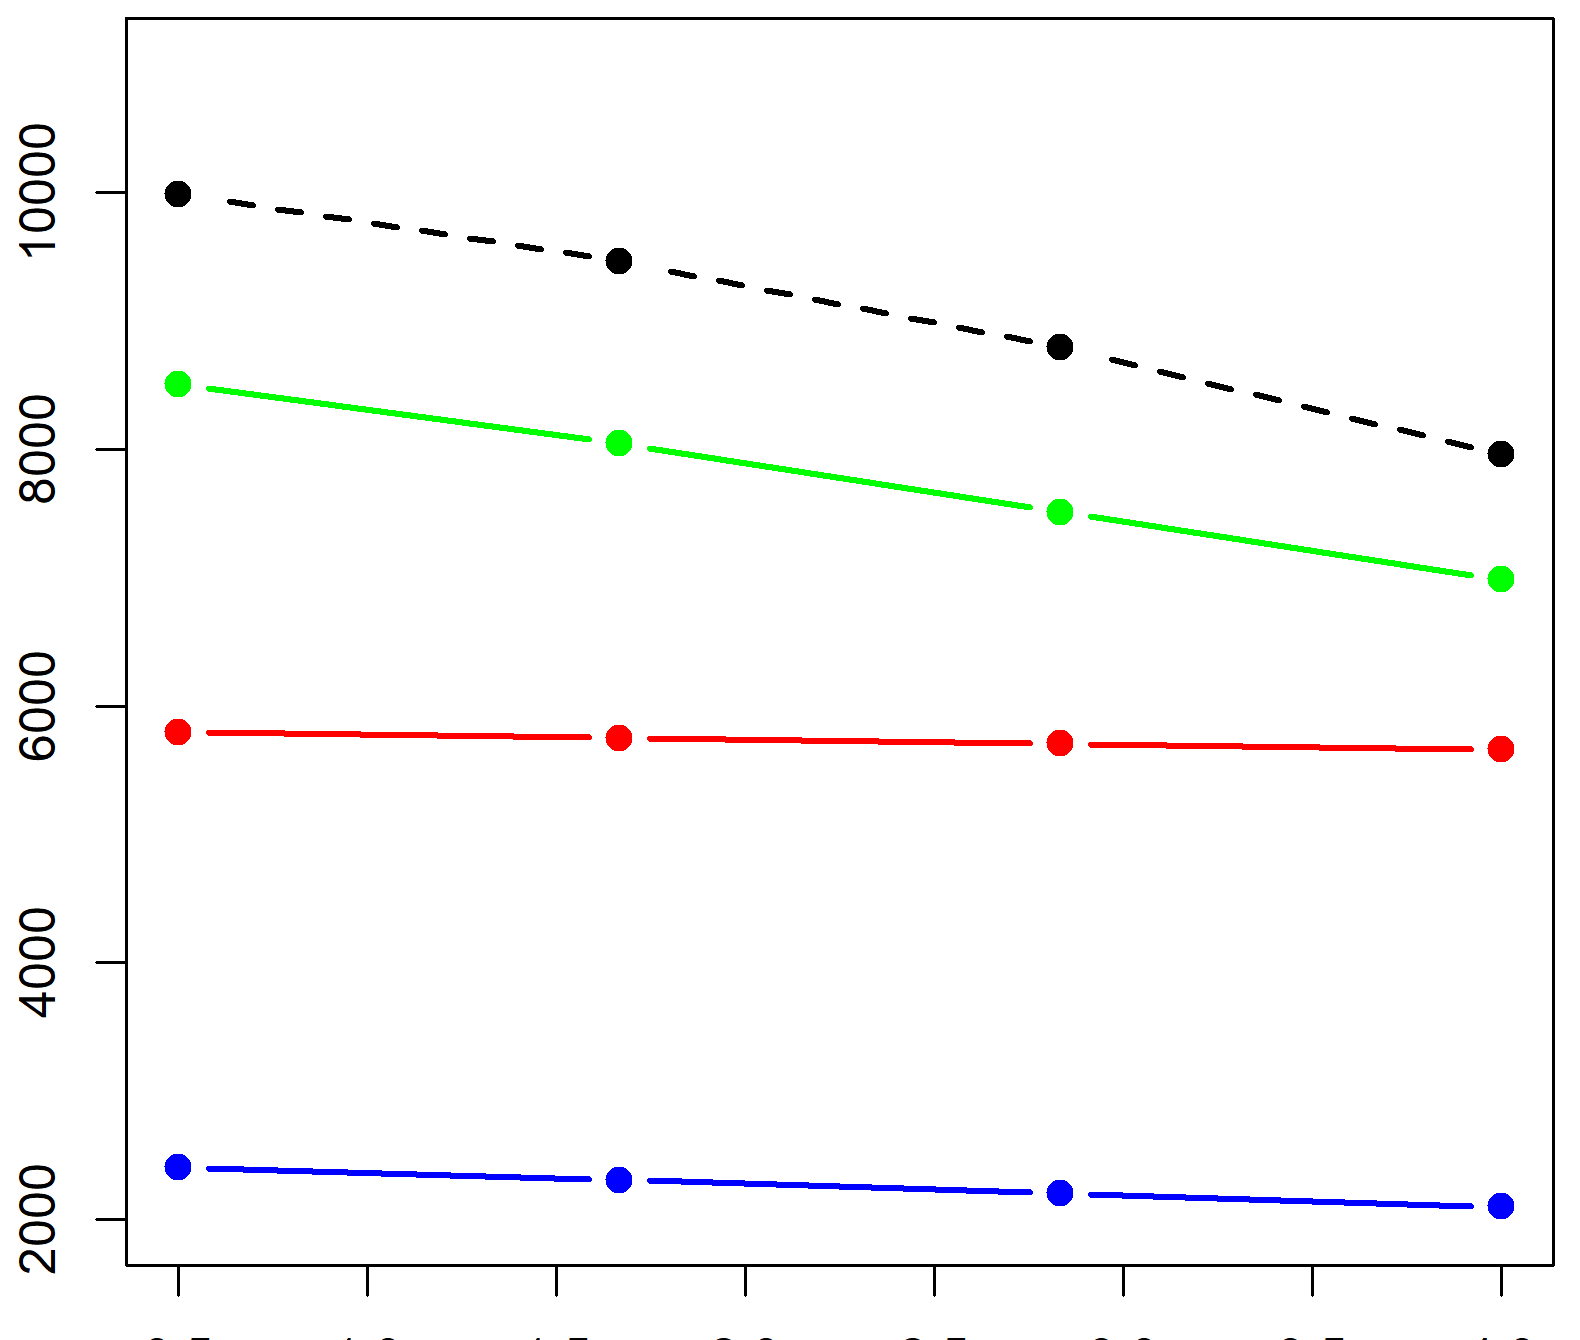
\includegraphics[scale=.6]{figures/example_figure.png}
    \label{fig:1}
\end{figure}

\medskip

\bibliography{references.bib} 

\end{document}